% !TEX encoding = UTF-8
% !TEX TS-program = pdflatex
% !TEX root = ../tesi.tex

%**************************************************************
\chapter{L'applicazione}
\label{cap:applicazione}
%**************************************************************

%\intro{Breve introduzione al capitolo}\\

\section{Introduzione alle grammatiche}
Zucchetti negli ultimi anni ha investito molto nella ricerca di una tecnologia che gli permettesse di interagire con i propri prodotti attraverso comandi vocali ed ora sta realizzando delle regole che consentono di generare un numero di \emph{grammatiche} potenzialmente infinito e capace di comprendere ed elaborare il linguaggio naturale.
Gli assistenti virtuali presenti sul mercato sono basati sul seguente concetto: provare ad interpretare l'input ricevuto anche se non corrisponde esattamente ad uno di quelli previsti a costo di commettere degli errori. Questa filosofia è mirata a dare all'utente la percezione di utilizzare uno strumento in grado di capire e ragionare in qualsiasi momento ed è già utilizzata in larga scala da aziende del calibro di Google, Amazon e Apple. Tuttavia, per le funzionalità offerte dalla maggior parte dei prodotti Zucchetti, tale principio non è applicabile poiché necessitano che la comprensione dell'input abbia margine di errore nullo. Un classico esempio è il trasferimento di denaro in cui se la comprensione del comando avviene in modo errato c'è il rischio di causare danni contingenti agli utenti. \\
Zucchetti ha perciò intrapreso una strada diversa sviluppando una tecnologia con l'obiettivo di massimizzare la precisione della comprensione dei comandi, accettando piuttosto di rigettarli. Essa consiste in regole molto semplici ed intuitive da applicare e riassunte in cinque operazioni chiave:
\begin{itemize}
	\item concatenazione di stringhe;
	\item scelta tra più stringhe;
	\item ripetizione di uno o più stringhe;
	\item opzionalità di una stringa;
	\item rilasciare una stringa a scelta dello sviluppatore in qualsiasi punto all'interno come segnale per l'elaborazione.
\end{itemize}
A partire da esse viene costruita una \emph{\gls{gramg}} che permette di interpretare un insieme finito di input che rappresentano il dominio della conversazione che si vuole intrattenere. La difficoltà principale è scegliere il corretto insieme delle possibili frasi che l'utente può pronunciare con l'obiettivo di ottenerne un numero molto elevato ma pertinente, eseguendo un'analisi probabilistica e statistica sul proprio contesto. Il problema infatti è che, qualora l'utente esprimesse una frase che differisca anche per una singola lettera da quelle generate dalla \emph{\gls{gramg}}, non sarebbe riconosciuta. \\
Un esempio semplice ma dimostrativo di una \emph{\gls{gramg}} che permette di interpretare alcune frasi di saluto è illustrato nella seguente immagine.

\begin{figure}[htbp]
	\begin{center}
		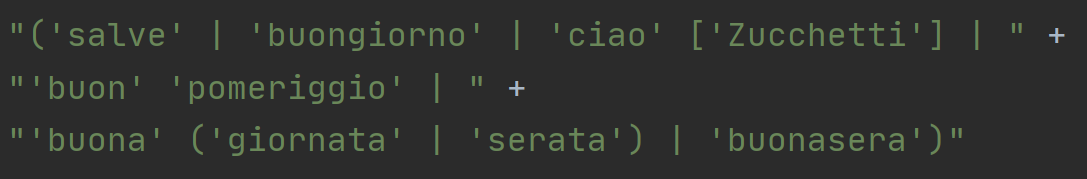
\includegraphics[height=2cm, width=\linewidth]{esempio-grammatica.PNG}
		\caption{Esempio di una grammatica}
	\end{center}
\end{figure}

\vspace{2cm}

Nonostante il loro principio di funzionamento sia relativamente semplice da comprendere, non sono altrettanto facili da interpretare se raggiungono grandi dimensioni, soprattutto per uno sviluppatore terzo che le dovrà riutilizzare in futuro. Per migliorare questo aspetto l'azienda ha quindi deciso di utilizzare i diagrammi \emph{\gls{rldg}}\glsfirstoccur come strumento di rappresentazione come si può vedere nella figura successiva.

\begin{figure}[htbp]
	\begin{center}
		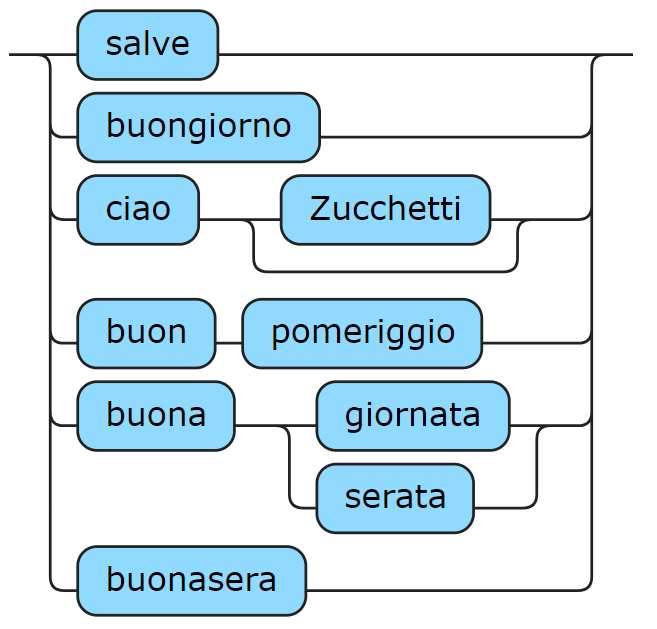
\includegraphics[height=6cm]{esempio-railroad.PNG}
		\caption{Esempio di una grammatica con railroad}
	\end{center}
\end{figure}

Risulta evidente infatti come questa raffigurazione sia molto più efficace e intuitiva. \\
Inoltre per l'applicazione effettiva della \emph{\gls{gramg}} sugli input dell'utente avviene attraverso un apposito \emph{\gls{parsg}}\glsfirstoccur che mi è stato consegnato dall'azienda per lo sviluppo del progetto. \\
Infine per riassumere gli aspetti positivi e negativi di questa tecnologia paragonata anche a quella attualmente utilizzata da Google, Alexa e Siri per i dati a disposizione, viene riportata la seguente tabella.

\begin{table}
	\begin{tabularx}{\textwidth}{|X|X|X|}
		\hline
		\textbf{Caratteristica} & \textbf{Zucchetti} & \textbf{Aziende concorrenti} \\\hline
		
		Precisione nella comprensione & Estrema precisione: quando afferma di aver compreso un frase ha la certezza di averlo fatto correttamente.  & Buona precisione: quando afferma di aver compreso una frase, non sempre è corretta. \\
		\hline
		Propensione alla comprensione & Comprende solo le frasi che lo sviluppatore mette a disposizione attraverso una \emph{\gls{gramg}}. & Cerca di interpretare anche frasi che non corrispondono esattamente alle configurazioni, talvolta commettendo degli errori. \\
		\hline
		Verbosità nello sviluppo & Poca verbosità in quanto, per costruzione, ad un aumento minimale vocaboli si ottiene un grande aumento delle frasi possibilmente interpretabili. & Dati non disponibili. \\
		\hline
		Facilità della sintassi & Molto facili da gestire in quanto è basata su regole semplici ma con grosse potenzialità & Dati non disponibili. \\
		\hline
		Prestazioni & Prestazioni molto elevate dovute ad un'ottima integrazione del \emph{\gls{parsg}} e all'esecuzione in locale senza quindi onere nella comunicazione. & Prestazioni altrettanto elevate ma con l'incognita dei tempi di latenza dovuti all'esecuzione in remoto del \emph{\gls{parsg}} per interpretare l'input. \\
		\hline
	\end{tabularx}
	\caption{Tabella di confronto tra la tecnologia Zucchetti e quella dei concorrenti per l'interpretazione del linguaggio naturale}
\end{table}

\section{Analisi dei requisiti}
	\subsection{Descrizione del problema}
	Durante l'attività di ricerca ed analisi sugli assistenti virtuali, in particolare nello sviluppo del \emph{\gls{pocg}} che fa uso di Alexa, è emerso un concetto importante, caratteristico anche del lavoro che sta svolgendo l'azienda: la conversazionalità. Essa rappresenta la capacità di intrattenere una conversazione da parte di un software simulando la presenza di una persona. \\
	Inoltre nella pianificazione del lavoro è inserita la costruzione di una \emph{\gls{nlug}} con relativa \emph{\gls{gramg}} che interpreti un insieme di frasi e dia una risposta ragionata sulla base di esse. \\
	È stato quindi deciso, in comune accordo con il tutor, di costruire un'applicazione che metta assieme la realizzazione di una propria \emph{\gls{nlug}} con capacità di conversazione finalizzata a soddisfare una determinata funzionalità e non limitata ad una coppia domanda-risposta. Il dominio di lavoro è simile a quello del \emph{\gls{pocg}} sviluppato con Alexa ovvero la data di nascita, solo che molto più completo. Le frasi pronunciabili dagli utenti per cui è prevista la comprensione sono  composte da:
	\begin{itemize}
		\item saluto iniziale opzionale;
		\item un insieme di frasi introduttive per esprimere la data di nascita nel formato giorno, mese e anno o, alternativamente, la data di compleanno nel formato giorno, mese;
		\item insieme di espressioni per la data di nascita e conseguentemente del sottoinsieme data di compleanno;
		\item insieme di frasi per riconoscere come data il giorno di Natale;
		\item insieme di frasi per riconoscere come data il primo giorno di un qualsiasi mese;
		\item insieme di frasi per interrompere in qualunque momento l'esecuzione;
		\item insieme di frasi per chiedere un eventuale aiuto sulle funzionalità dell'applicazione.
	\end{itemize}
	\subsection{Requisiti}
	Lo scopo principale è dimostrare la fattibilità di implementare la capacità conversazionale in una \emph{\gls{nlug}} costruita con la tecnologia sviluppata da Zucchetti. L'applicazione perciò si presenta sotto forma di \emph{\gls{pocg}} e non è quindi integrata in un software aziendale esistente. \\
	Analizzando più in dettaglio gli obiettivi da raggiungere, è stata stilata una lista di requisiti obbligatori la cui fattibilità è certa. Uno stra quelli emersi, invece, è stato inserito come opzionale poiché rappresenta un miglioramento ragionevolmente non implementabile nel tempo a disposizione.
	I requisiti obbligatori sono i seguenti:
	\begin{enumerate}
		\item costruzione dell'interfaccia utente:
			\begin{itemize}
				\item interfaccia grafica minimale che permetta all'utente di attivare il riconoscimento della voce;
				\item interfaccia vocale completa di tutti gli accessori studiati durante l'attività di ricerca. In input risulta essere una diretta conseguenza dello sviluppo della \emph{\gls{nlug}} mentre in output è progettata sulla base delle elaborazioni prodotte.
			\end{itemize}
		\item costruzione di una \emph{\gls{nlug}} che comprenda la data di nascita espressa dall'utente, esegua un'elaborazione e prepari una risposta adatta. Deve avere estrema precisione nella comprensione delle le frasi anche a costo di rigettarne alcune;
		\item implementazione della capacità conversazionale con relativa memoria che permetta di portare a compimento l'attività in esecuzione, dando maggiormente la percezione all'utente di dialogare con una persona. Più in dettaglio consiste nel richiedere i componenti mancanti della data di nascita o di compleanno affinché l'utente li fornisca in modo completo.
	\end{enumerate}
	Il requisito opzionale è il seguente:
	\begin{itemize}
		\item generalizzazione della grammatica in modo che permetta non solo di interpretare l'input dell'utente ma anche di generare la risposta sulla base dell'elaborazione.
	\end{itemize}
\section{Progettazione}
	\subsection{NLU}
	La \emph{\gls{nlug}} è il nucleo di tutto l'applicativo e la sua corretta progettazione è fondamentale. Essa consiste nella \emph{\gls{gramg}} generata dallo sviluppatore che interpreta l'input dell'utente e nella sua applicazione alle stringhe di testo. La \emph{\gls{gramg}} non è rappresentabile in un unico diagramma  in quanto ha dimensioni troppo elevate perciò sono illustrate le parti fondamentali. \\
	Il seguente diagramma rappresenta l'insieme di frasi per richiedere la data di nascita in cui prima viene detto il frammento di frase che corrisponde all'introduzione del contenuto come ad esempio "sono nato il" oppure "la mia data di nascita è" e successivamente il contenuto vero e proprio ovvero giorno, mese e anno in tutte le possibili combinazioni. 
		
	\begin{figure}[htbp]
		\begin{center}
			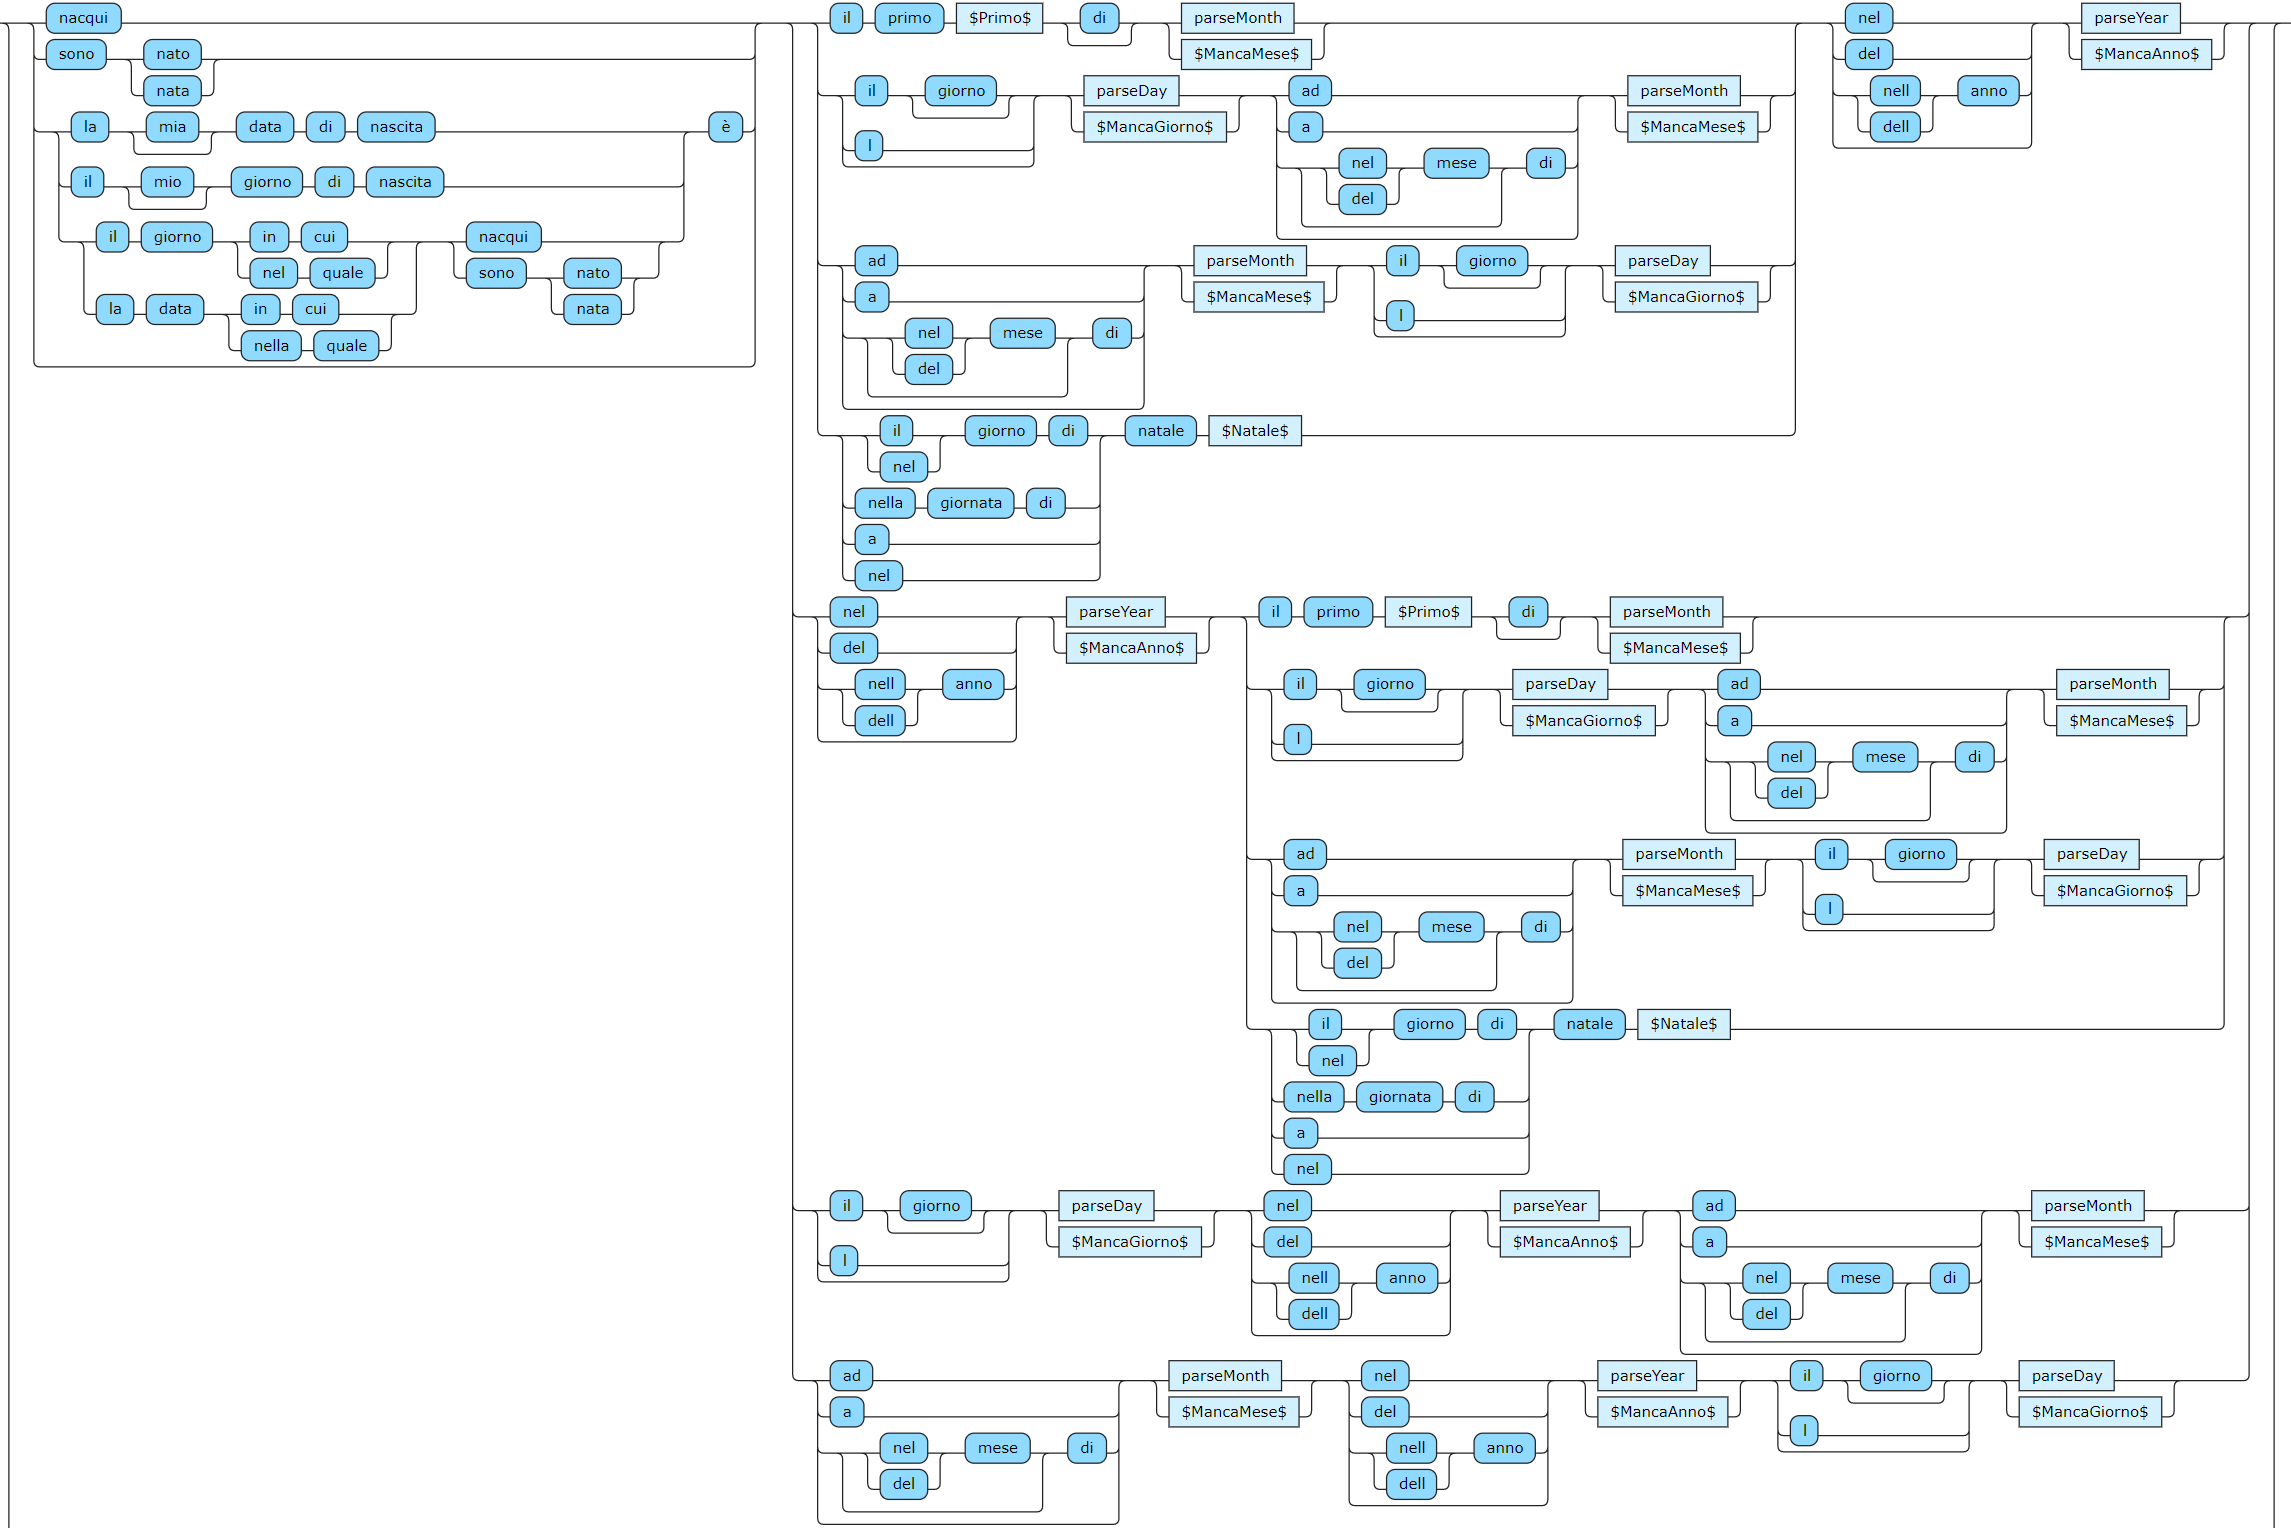
\includegraphics[height=10cm, width=\linewidth]{railroad_data_nascita.png}
			\caption{Diagramma railroad della grammatica per la data di nascita prima parte}
		\end{center}
	\end{figure}
	
	Nella figura successiva invece è rappresentato il diagramma \emph{\gls{rldg}} opposto in quanto prima prevede il contenuto ovvero giorno, mese e anno sempre in tutte le possibili combinazioni ed in seguito le sue frasi introduttive. Questo permette di riconoscere più versioni in cui l'utente può esprimere la data di nascita.
	
	\begin{figure}[htbp]
		\begin{center}
			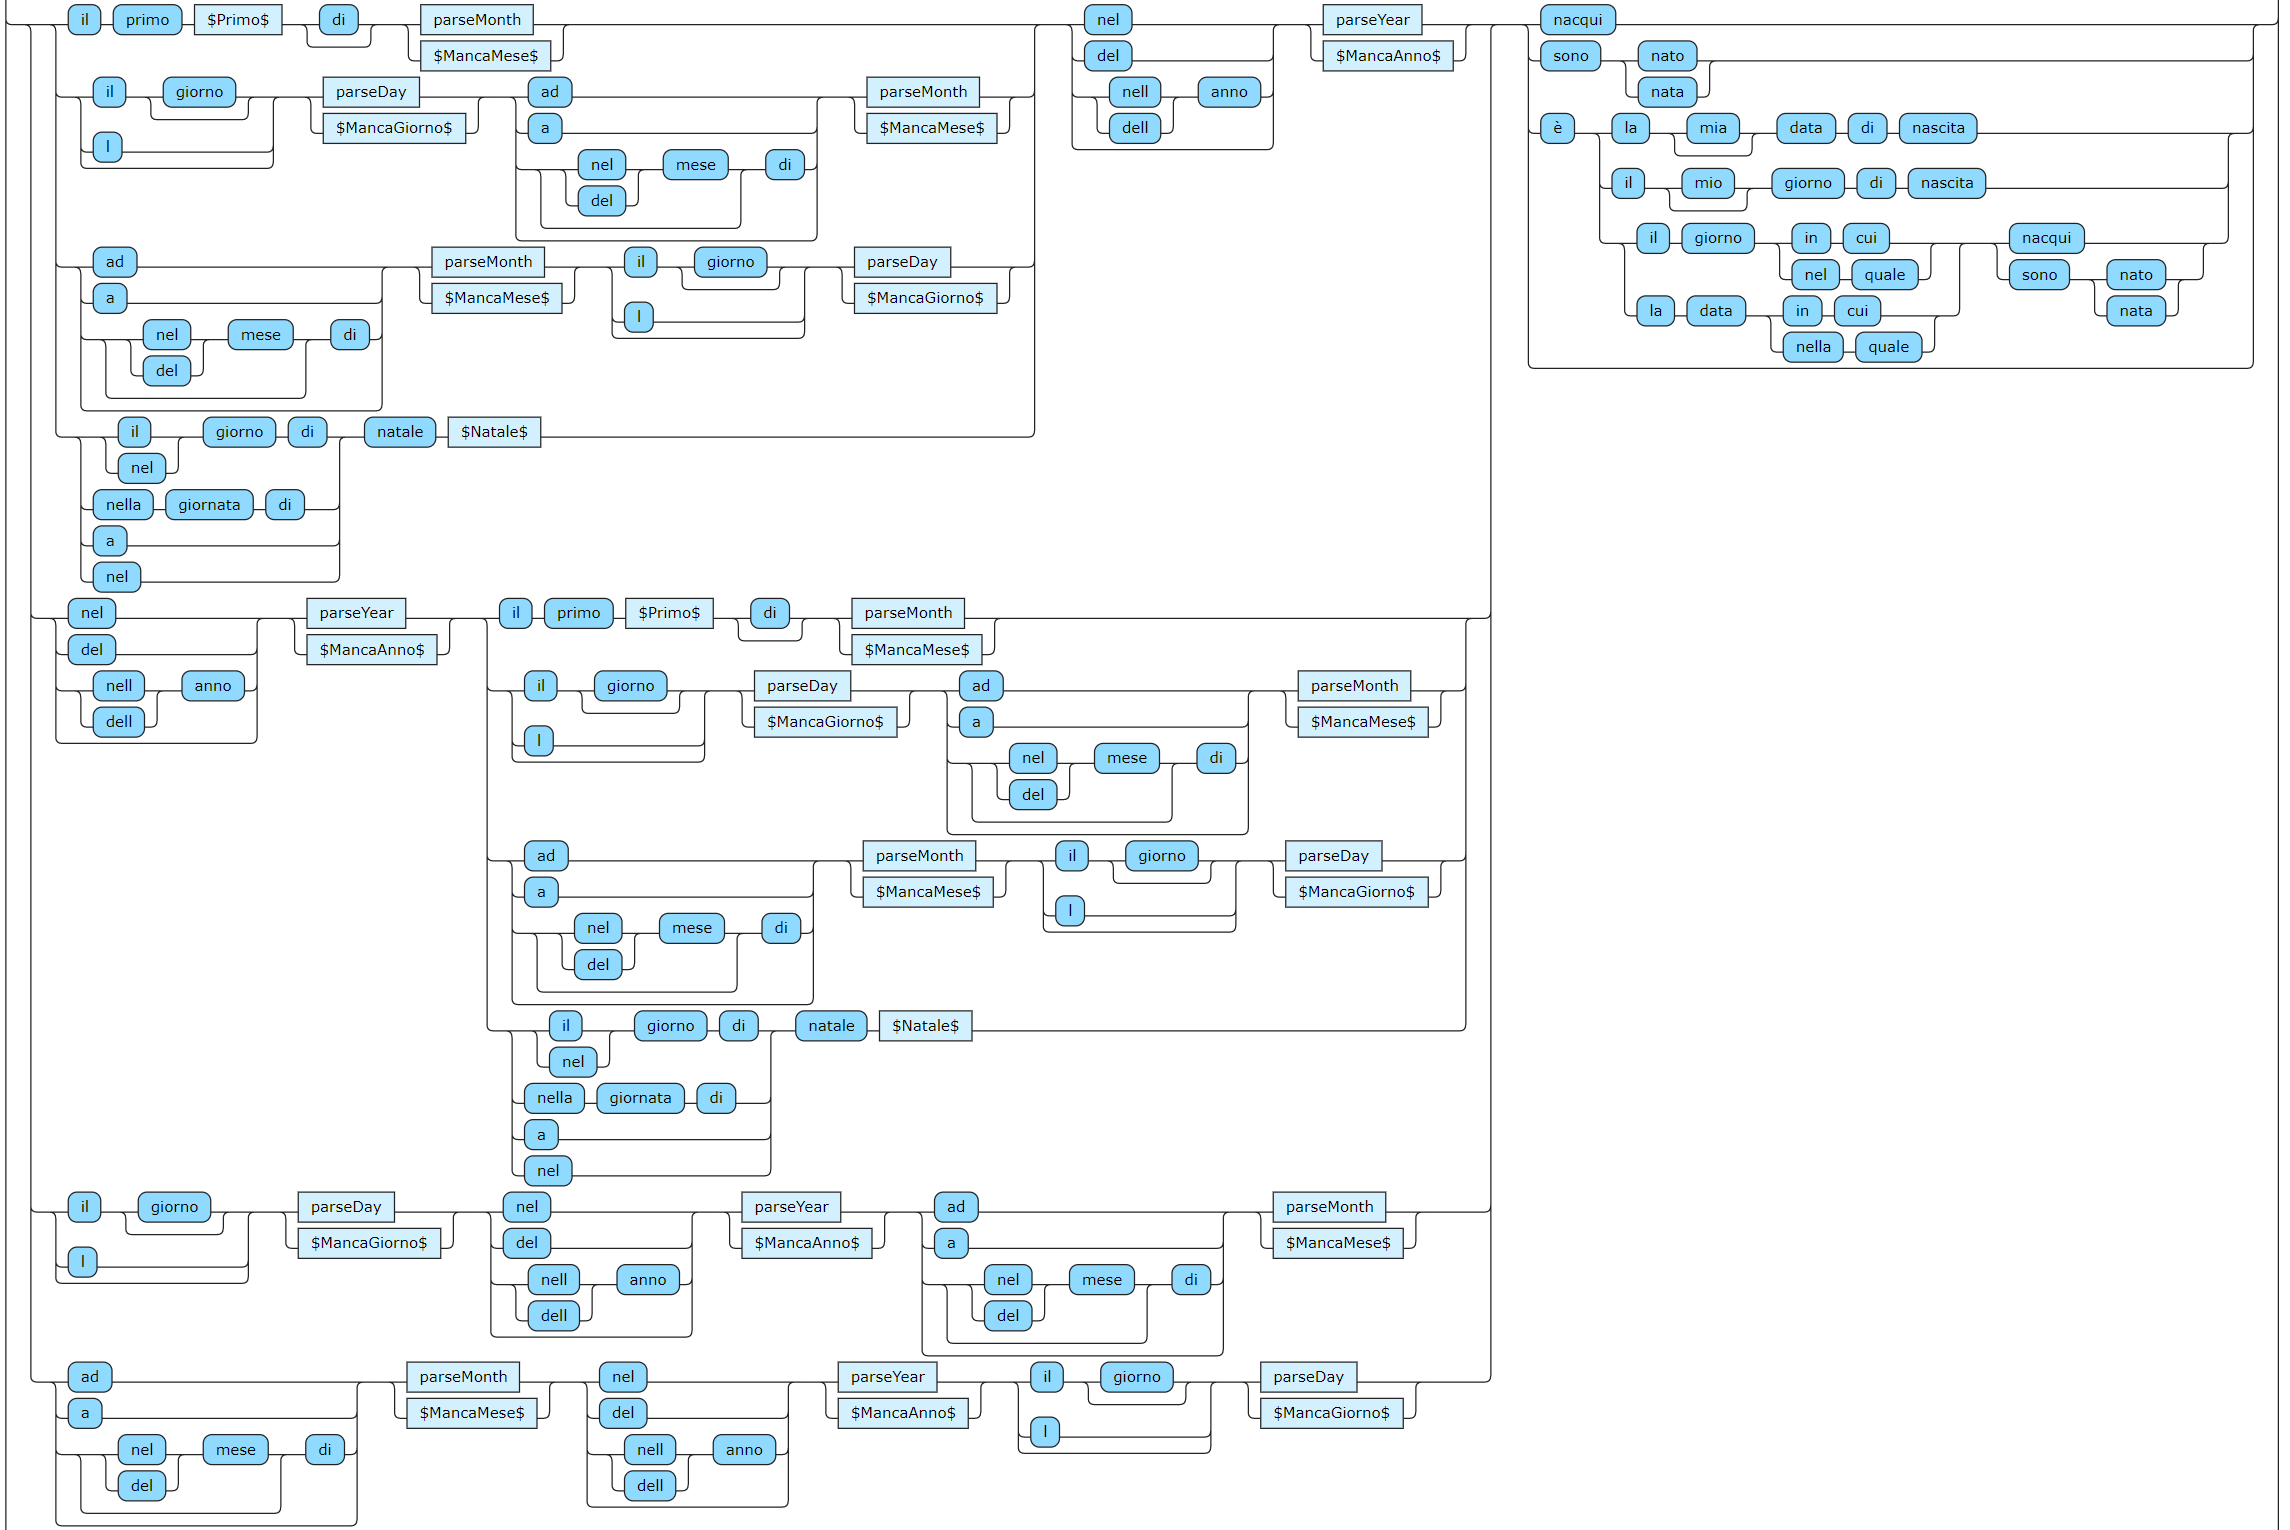
\includegraphics[height=10cm, width=\linewidth]{railroad_data_nascita_2.png}
			\caption{Diagramma railroad della grammatica per la data di nascita seconda parte}
		\end{center}
	\end{figure}

	Le due porzioni di \emph{\gls{gramg}} illustrate permettono globalmente di interpretare la data di nascita. Successivamente, seguendo lo stesso principio di separazione tra i frammenti di frase introduttivi e quelli di contesto, sono presentate le due porzioni di \emph{\gls{gramg}} che illustrano la data di compleanno, differente dalla precedente per l'assenza dell'anno. \\
	La figura seguente riporta la porzione che presenta prima la parte introduttiva e dopo quella di contenuto.
	
	\begin{figure}[htbp]
		\begin{center}
			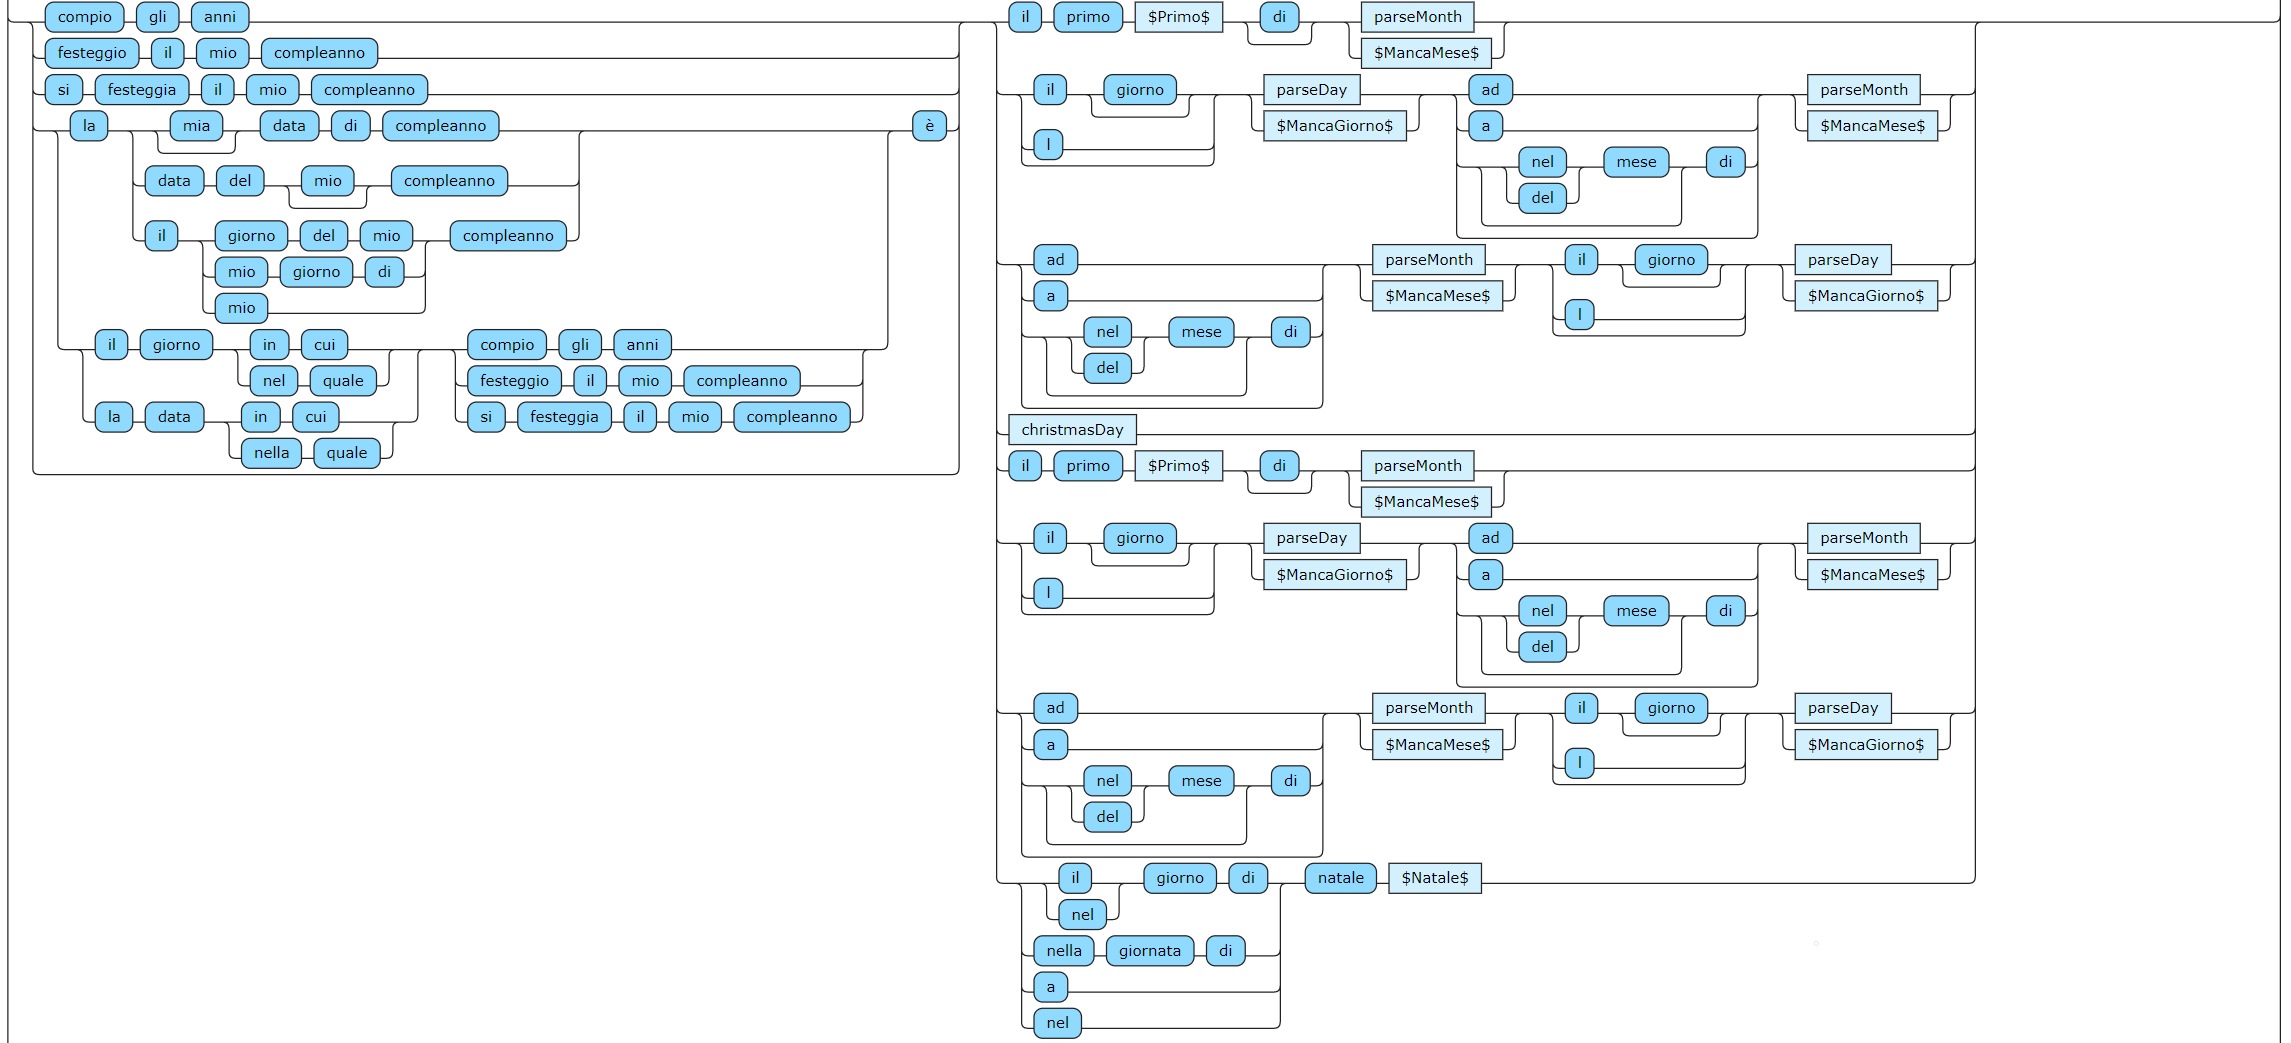
\includegraphics[height=8cm, width=\linewidth]{railroad_compleanno.png}
			\caption{Diagramma railroad della grammatica per il compleanno prima parte}
		\end{center}
	\end{figure}

	La prossima figura, invece, riporta la porzione che presenta prima la parte di contenuto e dopo quella introduttiva.
	\begin{figure}[htbp]
		\begin{center}
			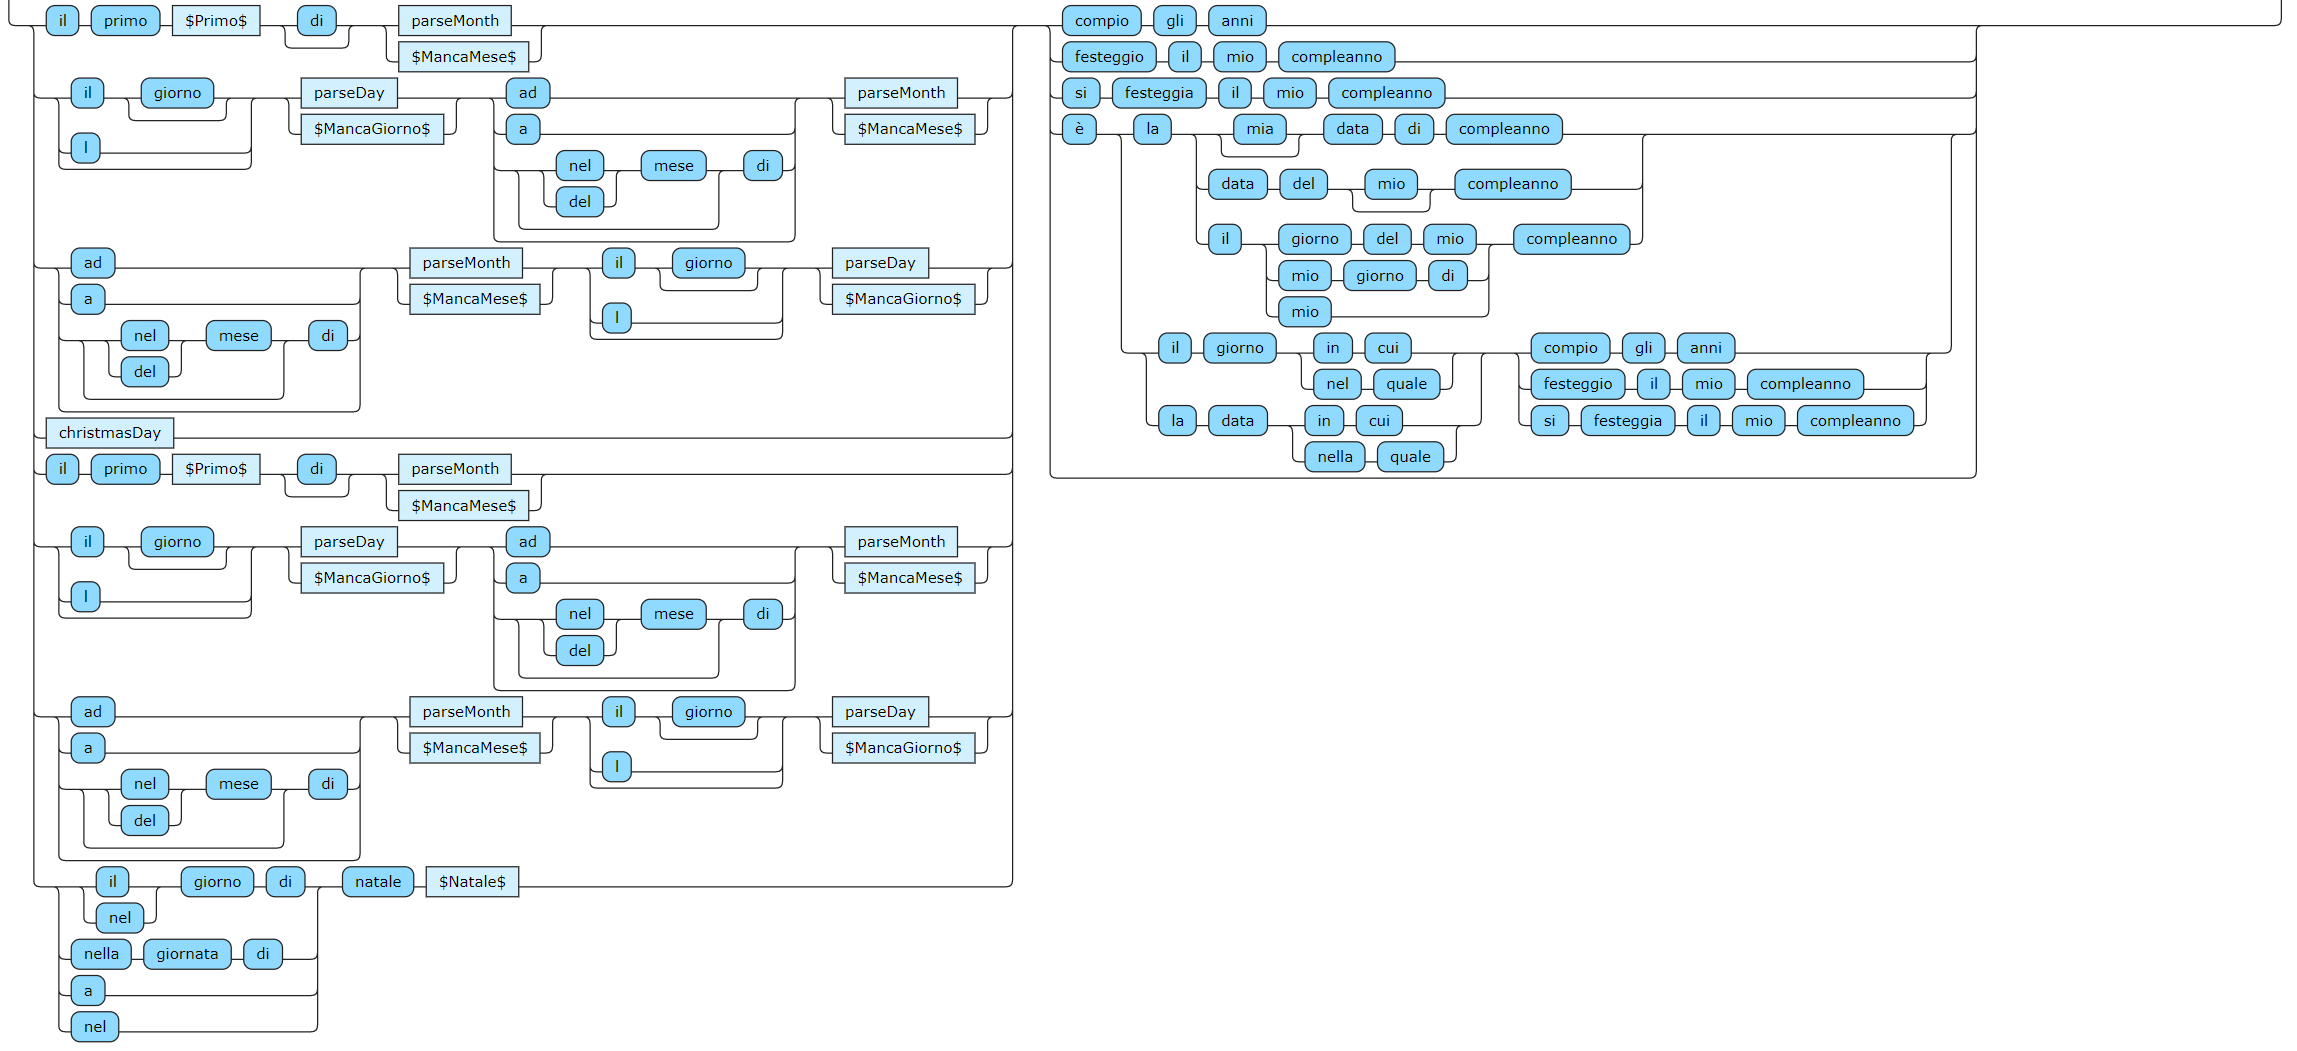
\includegraphics[height=8cm, width=\linewidth]{railroad_compleanno_2.png}
			\caption{Diagramma railroad della grammatica per il compleanno seconda parte}
		\end{center}
	\end{figure}

	\subsection{Capacità conversazionale}
	Per l'implementazione della capacità conversazionale il concetto fondamentale è la memoria. Infatti, mentre la \emph{\gls{nlug}} permette l'interpretazione del linguaggio naturale, la capacità conversazionale consente di mantenere il contesto durante l'intero dialogo. Ho deciso di tenere traccia dei dati che lo costituiscono all'interno di un oggetto che sarà resettato ad ogni nuova conversazione. In questo modo è possibile costruire delle risposte basate sul contesto per porre domande mirate ad ottenere gli eventuali dati mancanti ovvero giorno, mese e anno. \\
	La \emph{\gls{gramg}} descritta in precedenza è stata progettata anche per riconoscere singole parti di contenuto e di conseguenza viene riutilizzata anche per l'implementazione della conversazione. 
	\subsection{Interfaccia utente}
	La progettazione dell'interfaccia utente si articola in due parti:
	\begin{itemize}
		\item interfaccia grafica;
		\item interfaccia vocale.
	\end{itemize}
		\subsubsection{Interfaccia grafica}
		L'interfaccia grafica è stata progettata con un numero di elementi minimali all'interno ed è illustrata nella seguente immagine.
		\begin{figure}[htbp]
			\begin{center}
				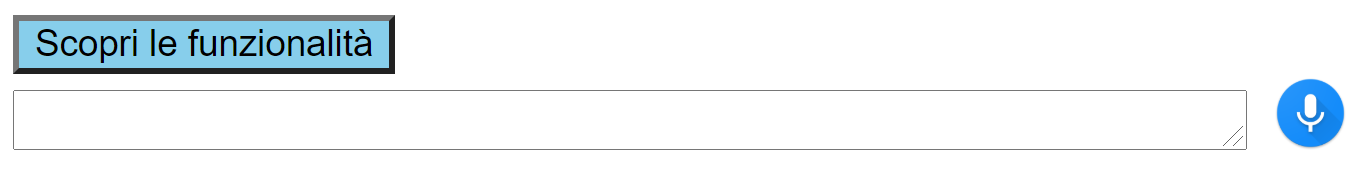
\includegraphics[height=1.7cm, width=\linewidth]{interfaccia-grafica.PNG}
				\caption{Interfaccia grafica dell'applicazione}
			\end{center}
		\end{figure}
	
		I componenti infatti sono un pulsante che permette all'utente di ascoltare le funzionalità fornite, un pulsante con l'immagine del microfono che attiva il riconoscimento vocale ed infine una casella di testo non editabile che permetta di visualizzare il comando che è stato riconosciuto.		
		\subsubsection{Interfaccia vocale}
		L'interfaccia vocale è stata progettata con l'obiettivo di garantire un'esperienza d'uso migliore possibile agli utenti. Ho utilizzato le nozioni apprese dalla documentazione degli assistenti virtuali analizzati per generare un'interfaccia vocale e sono:
		\begin{itemize}
			\item capire quali sono gli utenti che devono interagire con la propria applicazione. In questo caso ha importanza relativa in quanto si tratta di un \emph{\gls{pocg}};
			\item provare a costruire finestre di dialogo molteplice e provare quelle che risultano più naturali su un insieme di persone esterne. Nel mio caso l'ho provato con alcuni colleghi e persone esterne;
			\item scegliere una stile di conversazione che si adatti maggiormente al contesto della propria applicazione;
			\item dare una spiegazione iniziale di ciò che si può dire o fare in caso di interfaccia grafica ausiliaria;
			\item valutare l'utilizzo di un'interfaccia grafica di ausilio per mantenere meglio il contesto in caso sia corposo;
			\item gestire correttamente i possibili errori dovuti anche ad input scorretti dell'utente;
			\item dare la possibilità di aiutare l'utente in caso di difficoltà con frasi mirate;
			\item permette all'utente di interrompere l'esecuzione in qualsiasi momento senza bloccarlo.
		\end{itemize}		
		Tutti i componenti espressi nell'analisi sono quindi stati progettati. In particolare i comandi corrispondenti all'interruzione forzata dell'applicazione e alla richiesta d'aiuto che sono stati utilizzati risultano un'elaborazione di un sottoinsieme di quelli ricavati da un'analisi comportamentale di Zucchetti sugli utenti, qualora siano tranquilli e rilassati ma anche arrabbiati e agitati. \\
		Per gli input dell'utente l'interfaccia vocale è realizzata automaticamente a partire dalla progettazione della \emph{\gls{gramg}} per la quale sono comunque stati applicati i principi descritti mentre per l'output è stata personalizzata sulla base dell'elaborazione. Si è quindi deciso di fornire un set di frasi con significato uguale ma con una sintassi leggermente diversa da cui viene scelta al momento la frasi di input secondo un algoritmo pseudo-casuale.
\section{Codifica}

\section{Test}

\section{Sviluppi futuri}
Sarebbe stato possibile tenere traccia dei dati forniti dall'utente in modo permanente ad esempio all'interno di un database così che ad un nuovo utilizzo dell'utente l'applicazione si ricordasse di ciò che era stato detto precedentemente. Questo però pone alcuni vincoli quali un sistema di autenticazione dell'utente perciò diventa complesso.